\chapter{Frequency Reponse Curves}\label{ch:appB}

\begin{figure}[!h] 
\centering
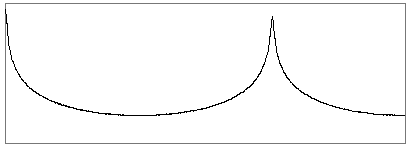
\includegraphics[width=1\textwidth]{comblowdelay}
\caption{\label{fig:comblowdelay} Comb filter with short delay.}
\end{figure}

\begin{figure}[!h] 
\centering
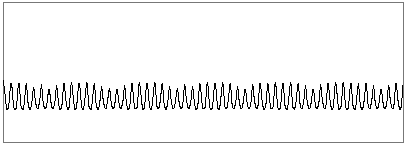
\includegraphics[width=1\textwidth]{combhighdelay}
\caption{\label{fig:combhighdelay} Comb filter with long delay.}
\end{figure}

\begin{figure}[!h] 
\centering
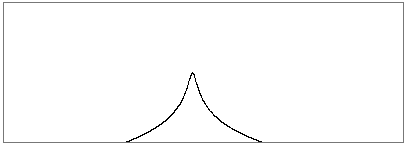
\includegraphics[width=1\textwidth]{bandpasslowbw}
\caption{\label{fig:bandpasslowbw} Bandpass filter with low bandwidth.}
\end{figure}

\begin{figure}[!h] 
\centering
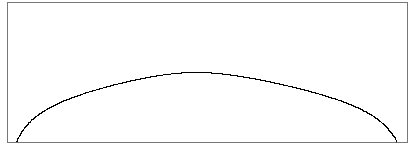
\includegraphics[width=1\textwidth]{bandpasshighbw}
\caption{\label{fig:bandpasshighbw} Bandpass filter with high bandwidth.}
\end{figure}

\begin{figure}[!h] 
\centering
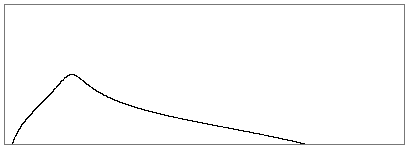
\includegraphics[width=1\textwidth]{bandpasslowf0}
\caption{\label{fig:bandpasslowf0} Bandpass filter with low centre frequency.}
\end{figure}

\begin{figure}[!h] 
\centering
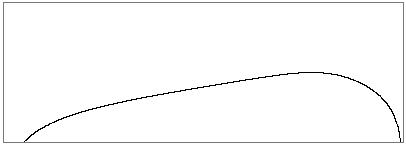
\includegraphics[width=1\textwidth]{bandpasshighf0}
\caption{\label{fig:bandpasshighf0} Bandpass filter with high centre frequency.}
\end{figure}

\begin{figure}[!h] 
\centering
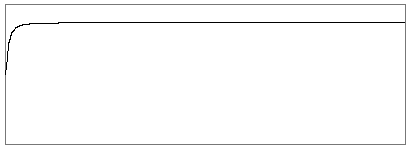
\includegraphics[width=1\textwidth]{highshelflowf0}
\caption{\label{fig:highshelflowf0} High-shelf filter with low cut-off frequency.}
\end{figure}

\begin{figure}[!h] 
\centering
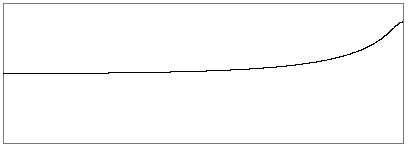
\includegraphics[width=1\textwidth]{highshelfhighf0}
\caption{\label{fig:highshelhighf0} High-shelf filter with high cut-off frequency.}
\end{figure}

\begin{figure}[!h] 
\centering
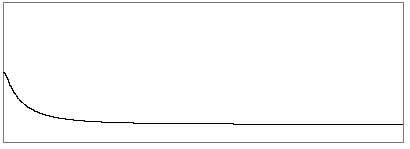
\includegraphics[width=1\textwidth]{highshelflowdbgain}
\caption{\label{fig:highshelflowdbgain} High-shelf filter with low decibel gain.}
\end{figure}

\begin{figure}[!h] 
\centering
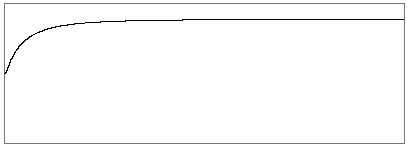
\includegraphics[width=1\textwidth]{highshelfhighdbgain}
\caption{\label{fig:highshelfhighdbgain} High-shelf filter with high decibel gain.}
\end{figure}

\begin{figure}[!h] 
\centering
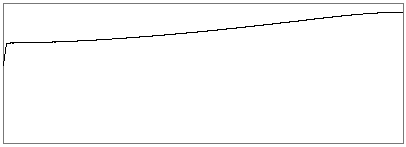
\includegraphics[width=1\textwidth]{highshelflowslope}
\caption{\label{fig:highshelflowslope} High-shelf filter with low slope variable.}
\end{figure}

\begin{figure}[!h] 
\centering
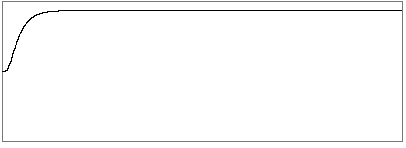
\includegraphics[width=1\textwidth]{highshelfhighslope}
\caption{\label{fig:highshelfhighslope} High-shelf filter with high slope variable.}
\end{figure}